\documentclass[14 pt, fleqn, pstricks]{extarticle}

	\usepackage[frenchb]{babel}
	\usepackage[utf8]{inputenc}  
	\usepackage[T1]{fontenc}
	\usepackage{amssymb}
	\usepackage[mathscr]{euscript}
	\usepackage{stmaryrd}
	\usepackage{amsmath}
	\usepackage{tikz}
	\usepackage[all,cmtip]{xy}
	\usepackage{amsthm}
	\usepackage{varioref}
	\usepackage{geometry}
	\usepackage{tabularx}
	\geometry{a4paper}
	\usepackage{lmodern}
	\usepackage{hyperref}
	\usepackage{array}
	 \usepackage{fancyhdr}
	 \usepackage{pstricks,pst-plot,pst-tree,pstricks-add}
\usepackage{pst-eucl}% permet de faire des dessins de géométrie simplement
\usepackage{pst-text}
\usepackage{pst-node,pst-all}
\usepackage{pst-func,pst-math,pst-bspline,pst-3dplot}  %%% POUR LE BAC %%%
	 \usepackage{float}\usepackage{setspace}
\setlength{\mathindent}{1cm}
\renewcommand{\theenumi}{\alph{enumi})}
	\pagestyle{fancy}
	\theoremstyle{plain}
	\fancyfoot[C]{} 
	\fancyhead[L]{}
	\fancyhead[R]{}\geometry{
 a4paper,
 total={170mm,257mm},bottom = 0pt, top = 10pt
 }
	
	
	\title{Contrôle chapitre 6}
	\date{11 mars 2025}
	\begin{document}
	 
	 \maketitle
\subsection*{Exercice 1 (3 points)}	 
	 
On considère une fonction $g$ dont un tableau de valeurs est le suivant : \begin{figure}[H]
\center
$\begin{array}{|c|c|c|c|c|c|}
\hline
 x &  -3 & -1 & 4 & 8  &  2 \\
\hline
g(x)&  5 & -3  & -4 & 14 &   8   \\
\hline
\end{array}$
\end{figure}	 

\begin{enumerate}
\item Donnez une image de $8$ par $g$. 
\item Donnez un antécédent de $8$ par $g$. 
\item Donnez un nombre tel que $g(x)= - x$.
\end{enumerate}


\subsection*{Exercice 2 (10 points) }	 
	 
On considère le programme de calcul suivant : 
\begin{itemize}
\item[>] Prendre un nombre
\item[>] Le multiplier par 2
\item[>] Retirer 4
\item[>] Multiplier par le nombre de départ 
\item[>] Ajouter 6
\end{itemize}
\begin{enumerate}
\item (2 pts) On note $h(x)$ le résultat du programme lorsqu'on choisit le nombre $x$ au départ. Donnez une expression algébrique de $h(x)$.
% x(2x-4)+6
\item (1 pt) Calculez l'image de $-1$ par $h$. 
\item (1 pt) Calculez l'image de $\frac12$ par $h$.
\item (2 pts) Remplir le tableau suivant : 
	 
\begin{figure}[H]
\center
$\begin{array}{|c|c|c|c|c|c|}
\hline
 x &  3 & -5 & \frac12 &  -\frac23  &   \\
\hline
h(x)&   & & & & 12   \\
\hline
\end{array}$
\end{figure}
\item (2 pts) Développez et réduire l'expression de $h(x)$. \item (2 pts)  Montrer que le résultat du programme de calcul est toujours pair.
\end{enumerate} 

\newpage
\subsection*{Exercice 3 (7 points) }

\medskip

On donne le programme de calcul suivant : 

\begin{center}
\begin{tabularx}{0.6\linewidth}{|X|}\hline
$\bullet~~$Choisir un nombre\\
$\bullet~~$Ajouter 1 \\
$\bullet~~$Élever le résultat au carré\\
$\bullet~~$Soustraire au résultat le carré du nombre de départ\\ \hline
\end{tabularx}
\end{center}

\smallskip
\begin{enumerate}
\item (1 pt) Montrer que lorsqu'on choisit le nombre 2 au départ, on obtient le nombre 5 au final.
\item (1 pt) Quel résultat obtient-on lorsqu'on choisit au départ le nombre $-3$ ? 
\item (1 pt) On définit une fonction $f$ qui, à tout nombre $x$ choisi à l'entrée du programme, associe le résultat obtenu à la fin de ce programme. Exprimer $f(x)$ en fonction de $x$.

%\[\text{Ainsi, pour tout }\:x, \text{on obtient } \:f(x) = (x + 1)^2 - x^2\]

 

\item (4 pts) Dans chaque cas, une seule réponse est correcte. Pour chacune des questions, écrire sur la copie le numéro de la question et la bonne réponse. 
Aucune justification n'est demandée. 

\begin{center}
\begin{tabularx}{\linewidth}{|m{4cm}|*{3}{>{\centering \arraybackslash}X|}}\hline
\textbf{Question}&   \textbf{Réponse A}&   \textbf{Réponse B}&   \textbf{Réponse C}\\ \hline   
\textbf{1.~~} La représentation graphique de la fonction $f$ est:&\small  La représentation A&\small    La représentation B&\small La représentation C\\ \hline
\textbf{2.~~} En utilisant la représentation A, l'image de 1 par la fonction  représentée est:& 4   &$-2$&0\\ \hline
\textbf{3.~~} En utilisant la représentation B, l'antécédent de 3 par la fonction représentée est :&$-1$   &$-5$&   2\\ \hline
\end{tabularx}

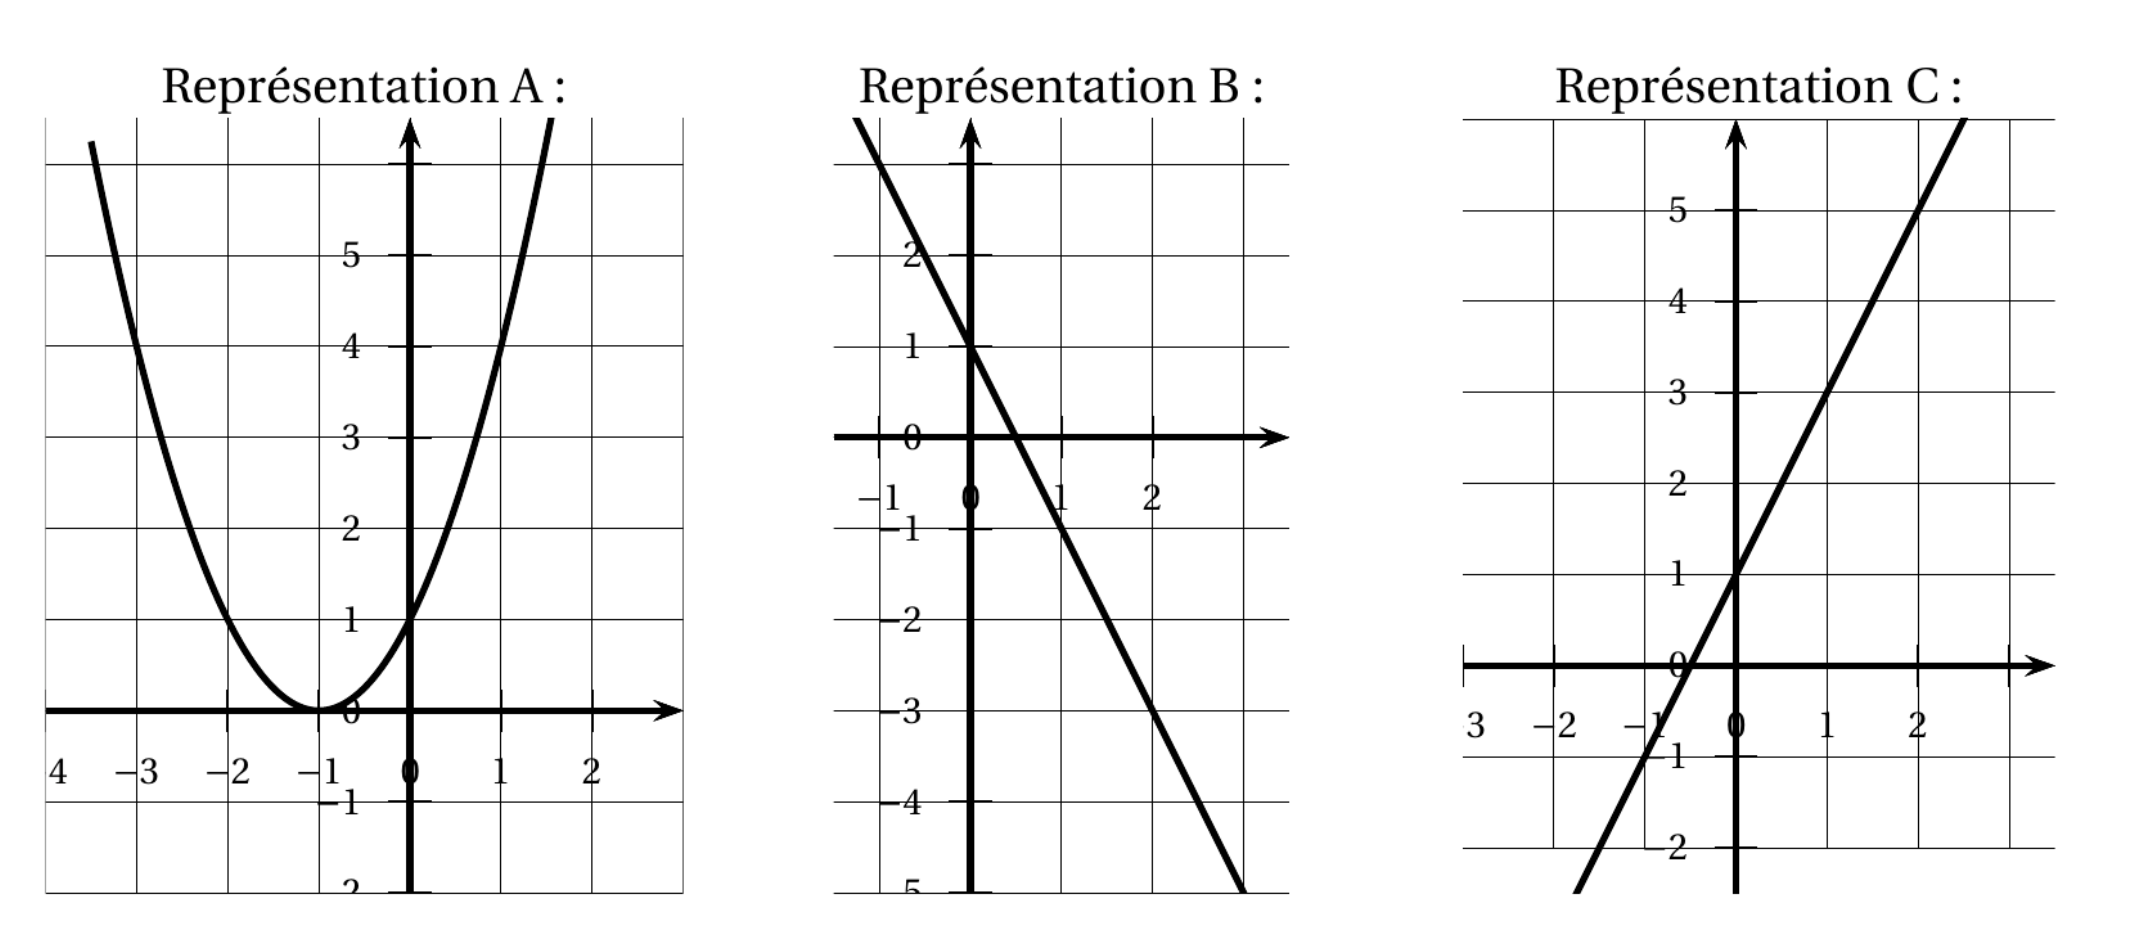
\includegraphics[scale=.45]{Figures}
 
\end{center}
\end{enumerate}
    

 	\end{document}







